% @out_file dokumentace.tex
% @author Štěpán Faragula
% @brief Dokumentace semestrální práce z předmětu KIV/MBKZ.
% @version 1.0
% @date 2024-05-01

% Document
\documentclass[12pt]{report}

% Čeština
\usepackage[utf8]{inputenc}
\usepackage[T1]{fontenc}
\usepackage[czech]{babel}

% Formát dokumentu
\usepackage{amsmath}
\usepackage{caption}
\usepackage{textcomp}
\usepackage{xspace}
\usepackage{parskip}
\usepackage[hidelinks]{hyperref}

% Graphics
\usepackage{graphicx}
\graphicspath{{img/}}
\usepackage{fancyvrb}
\usepackage[
left=30mm, 
right=30mm, 
top=30mm, 
bottom=30mm,
]{geometry}

% Vychytávky
\usepackage{lipsum}								% Lorem impsum
\usepackage{pdflscape}							% Landscape
\usepackage{menukeys}							% Klavesy
\usepackage{algorithm}							% Algoritmus
\usepackage[noend]{algpseudocode}				% Pseudokod
\usepackage{dirtree}							% Adresarova struktura
												% Tabulky pomoci https://www.tablesgenerator.com/
												

\usepackage{titlesec}
\titleformat{\chapter}{}{\bf\LARGE\thechapter~~~}{0em}{\bf\LARGE}

\newcommand\indentt[1]{						
	\setlength\parindent{5mm}
	#1
	\setlength\parindent{0mm}
}	


% ---------------------	
% Begin
% ---------------------	
\begin{document}


	% ---------------------		
	% Titulní strana
	% ---------------------	
	\begin{titlepage}
		\centering
		\Large
		
		
\includegraphics[width=.7\textwidth]{fav}
		
		\vspace{15mm}
		{\Huge\bfseries Procvičování matematiky}

		\vspace{5mm}
		{\LARGE Katedra informatiky a výpočetní techniky}
		{\LARGE Semestrální práce z předmětu KIV/MBKZ}
		
		\vfill
		\raggedright
		Štěpán Faragula\\
		A21B0119P\\
		farag844@students.zcu.cz
		\hfill 
		\today
	\end{titlepage}

	
	% ---------------------	
	% Obsah
	% ---------------------	
	\tableofcontents


	% ---------------------	
	% Zadání	
	% ---------------------	
	\chapter{Zadání}
	Cílem této semestrální práce je vytvořit aplikaci na procvičování matematiky. Přestože již existují podobné aplikace, zatím se mi nepodařilo najít takovou, která by podporovala počítání se zápornými čísly. Zadání jsem si tedy zvolil vzhledem k osobním potřebám.
	
	Cvičení bude fungovat na jednoduchém principu. Uživateli bude představen náhodně vygenerovaný příklad, ve kterém bude jedna neznámá hodnota. Následně bude muset uhodnout správnou hodnotu, a to buď výběrem ze 4 možností, nebo vlastnoručním vyplněním čísla. Jeden z těchto módů by mohl být pojat ve stylu hry, přičemž se bude navyšovat skóre podle správně vypočítaných příkladů. 
	
	Při vývoji bude kladen důraz na přizpůsobitelnost parametrů. Aplikace bude umět měnit volbu rozsahu, ve kterém se mohou čísla vyskytovat, spolu s dalšími možnostmi.



	% ---------------------			
	% Programátorská dokumentace
	% ---------------------	
	\chapter{Programátorská dokumentace}
	Aplikace byla vyvíjena pro platformu Android s úrovní API 24 a vyšší. K tomu bylo použito vývojové prostředí Android Studio.

	Bylo implementováno celkem 5 tříd \texttt{Activity}, každá s vlastním rozhraním \texttt{ContentView}. Ve zkratce se jednotlivé aktivity zabývají následujícím:
	\begin{itemize}
		\item \texttt{Menu} - vstupní bod programu
		\item \texttt{Exercise} - první mód, 4 možné odpovědi
		\item \texttt{Challenge} - druhý mód, ruční zadávání výsledku
		\item \texttt{Settings} - nastavení parametrů
		\item \texttt{About} - stručné informace o aplikaci
	\end{itemize}

	U náhodného generování příkladů se nejprve zvolí matematická operace a jedno náhodné číslo z rozsahu. Další dvě čísla jsou dopočítána. Následně se zvolí, které z čísel by~mělo představovat neznámou hodnotu. V prvním módu se ještě vypočítají 3 nesprávné hodnoty, které jsou ukázány spolu se správnou. U násobení a dělení se nevyskytují příklady obsahující 0. Je to kvůli nejednoznačnému výsledku u násobení a neplatné operace u~dělení.
	
	Nastavení se ukládá do \texttt{SharedPreferences}. Na začátku každého cvičení se přečtou tato uložená data. V případě, kdy neexistují, načtou se výchozí hodnoty. U rozsahů matematických operací je nutné zadat taková čísla, aby mezi nimi byla vzdálenost alespoň 3, protože to algoritmus předpokládá.
	
	Aplikace také podporuje zobrazení uživatelského rozhraní v anglickém nebo českém jazyce spolu s barevným schématem podle nastavení systému Android. 
	

	% ---------------------	
	% Uživatelská dokumentace
	% ---------------------	
	\chapter{Uživatelská dokumentace}
	\section{Hlavní menu}	
	Zobrazí se po spuštění aplikace, slouží k navigaci.
	
	\begin{figure}[ht]
		\centering
		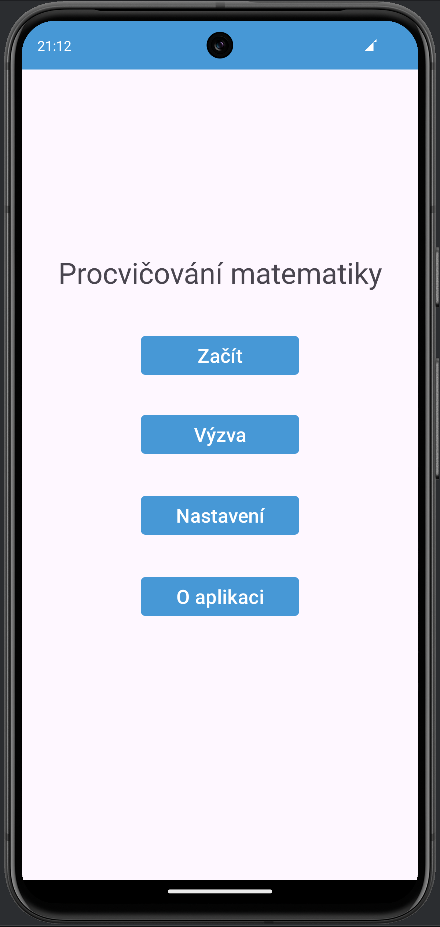
\includegraphics[height=0.9\textwidth]{img/menu}
		\label{fig:menu}
	\end{figure}
	
	\newpage
	\section{Procvičování}
	Uživateli se zobrazí náhodně vygenerovaný příklad spolu se 4 různými možnostmi. Další příklad se zobrazí po vybrání správného výsledku, přičemž se špatné odpovědi podbarví červeně. Na výběr je neomezený čas a po uhodnutí výsledku následuje vteřinová prodleva, která jej zvýrazní. Po určitém počtu příkladů se zobrazí hláška shrnující průběh cvičení. Po stisknutí tlačítka zpět na mobilu se zobrazí dialog, který musí být znovu potvrzen. Uživatel tak okamžitě neztratí postup při jeho nechtěném stisknutí.
	
	\begin{figure}[ht]
		\centering
		\begin{minipage}{.5\textwidth}
			\centering
			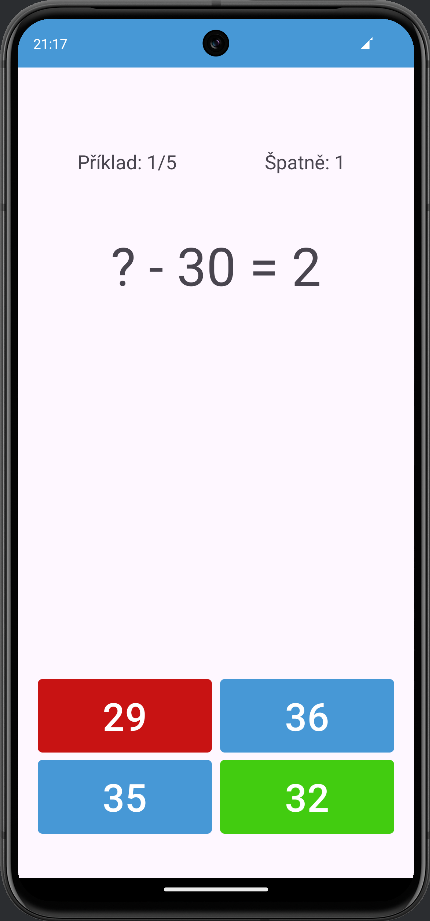
\includegraphics[height=1.7\textwidth]{img/exercise_1}
			\label{fig:exercise_1}
		\end{minipage}%
		\hfill
		\begin{minipage}{.5\textwidth}
			\centering
			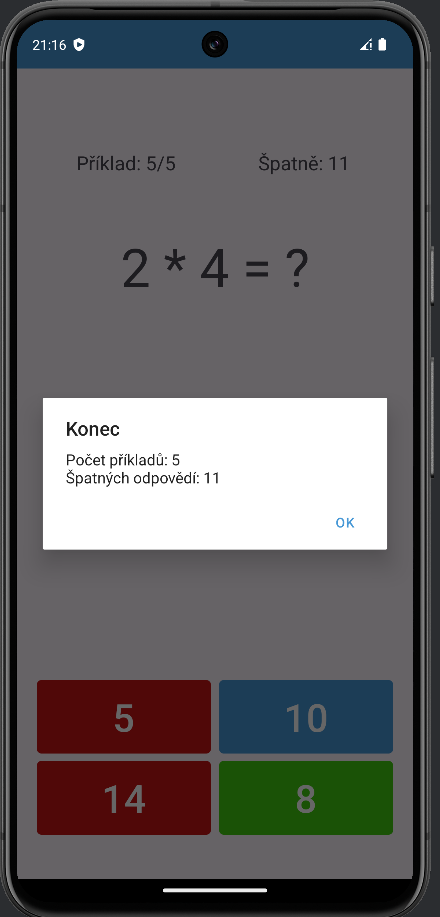
\includegraphics[height=1.7\textwidth]{img/exercise_2}
			\label{fig:exercise_2}
		\end{minipage}
	\end{figure}
	
	\newpage
	\section{Výzva}
	U výzvy musí uživatel zadávat všechny výsledky ručně. Skóre představuje počet doposud správně vypočítaných příkladů. Po odeslání čísla se na jednu vteřinu zobrazí barevný čtverec obsahující řešení. Pokud je odpověď špatná, výzva končí. Podle dosaženého skóre je zobrazena jedna z 5 vět, která by měla uživatele motivovat.
	
	\begin{figure}[ht]
		\centering
		\begin{minipage}{.5\textwidth}
			\centering
			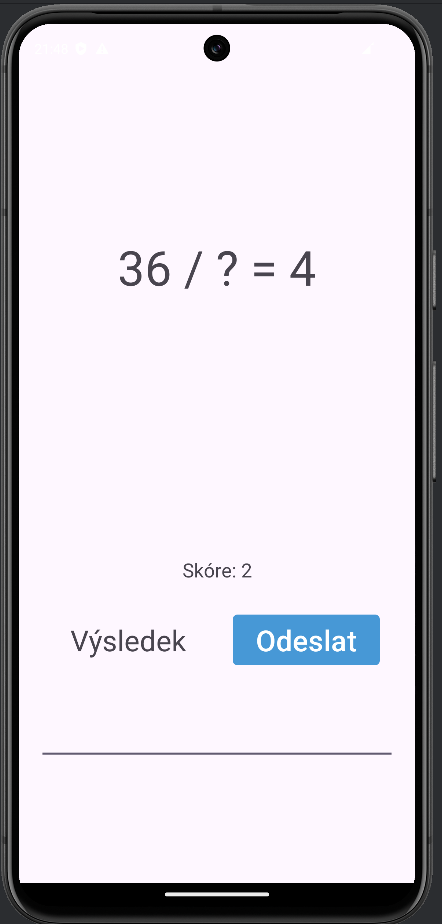
\includegraphics[height=1.7\textwidth]{img/challenge_1}
			\label{fig:challenge_1}
		\end{minipage}%
		\hfill
		\begin{minipage}{.5\textwidth}
			\centering
			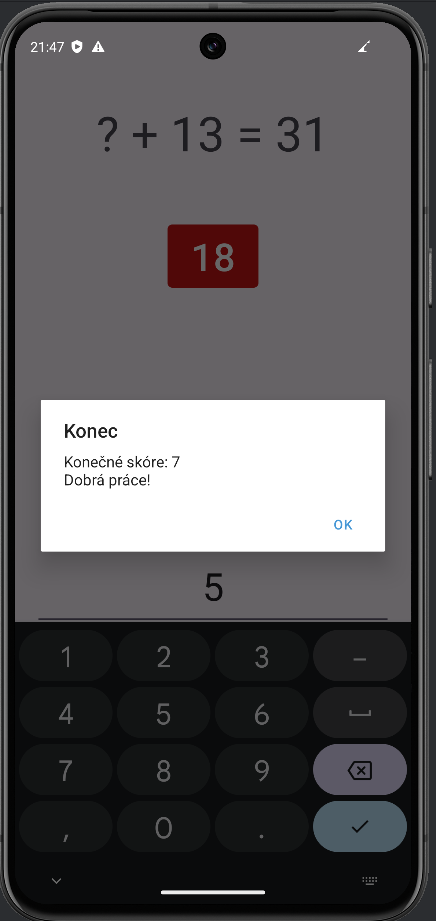
\includegraphics[height=1.7\textwidth]{img/challenge_2}
			\label{fig:challenge_2}
		\end{minipage}
	\end{figure}
	
	\newpage
	\section{Nastavení}
	Aplikace umožňuje měnit průběh cvičení. Provedené změny se budou týkat obou módů. Je možné měnit, na jaké pozici se~bude vyskytovat otazník a jaké operace by měly být procvičovány. Číselný rozsah operací může jít i do záporných hodnot. Dále je možné zvolit tmavý nebo světlý vzhled aplikace. Ve výchozím nastavení je určen systémem Android. Všechny možnosti se ukládají pomocí \texttt{SharedPreferences}. Uživatelský vstup je zabezpečen proti neplatným hodnotám.
	
	\begin{figure}[ht]
		\centering
		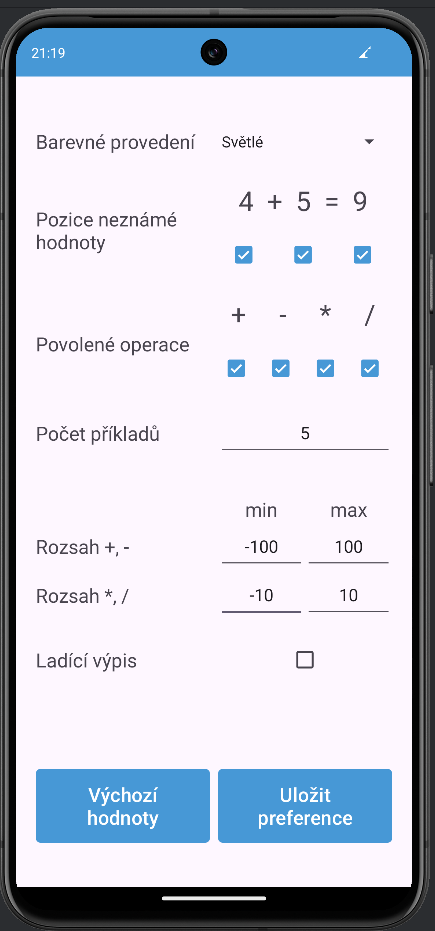
\includegraphics[height=0.9\textwidth]{img/settings}
		\label{fig:settings}
	\end{figure}
	
	\newpage
	\section{O aplikaci}
	Zde jsou vypsány základní informace o aplikaci.
	
	\begin{figure}[ht]
		\centering
		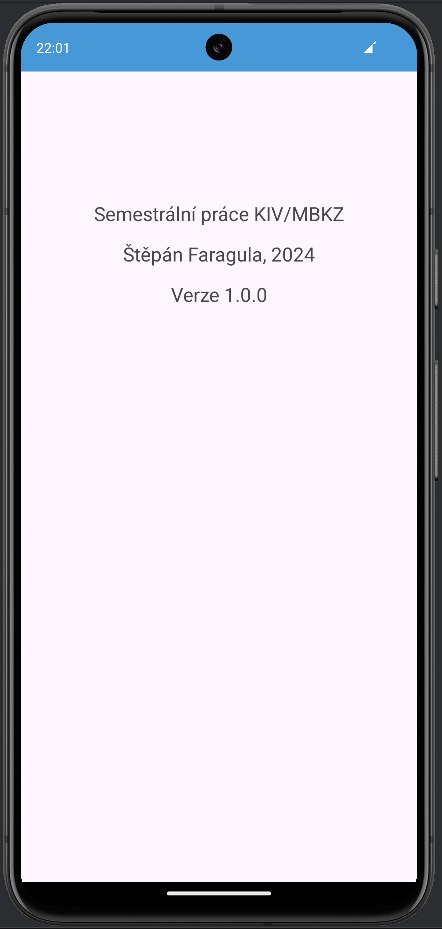
\includegraphics[height=0.9\textwidth]{img/about}
		\label{fig:about}
	\end{figure}
	
	\newpage
	\section{Lokalizace a přenositelnost}
	Uživatelské rozhraní umí přizpůsobit svůj jazyk a barevný motiv podle systému. Momentálně je aplikace přeložena do češtiny a angličtiny. Komponenty jsou adaptivní, dokážou se škálovat podle různých velikostí displejů. Po otočení telefonu se zobrazení nemění. 
	
	\begin{figure}[ht]
		\centering
		\begin{minipage}{.5\textwidth}
			\centering
			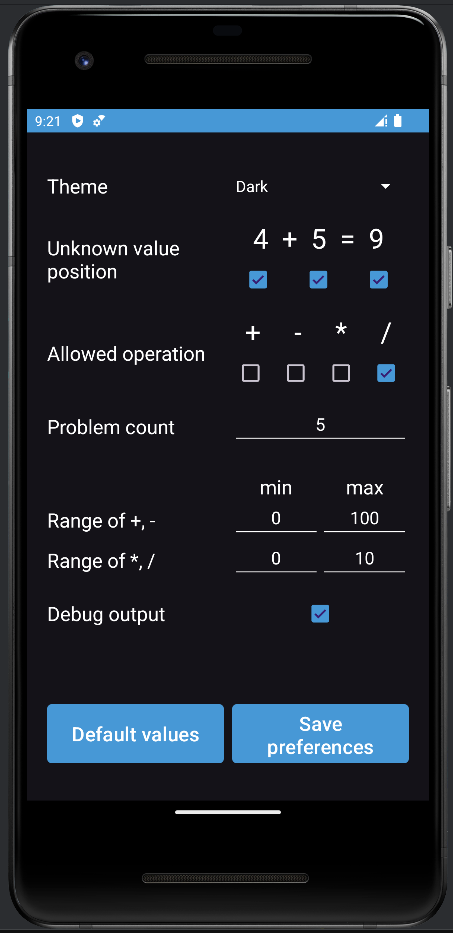
\includegraphics[height=1.7\textwidth]{img/dark_1}
			\label{fig:dark_1}
		\end{minipage}%
		\hfill
		\begin{minipage}{.5\textwidth}
			\centering
			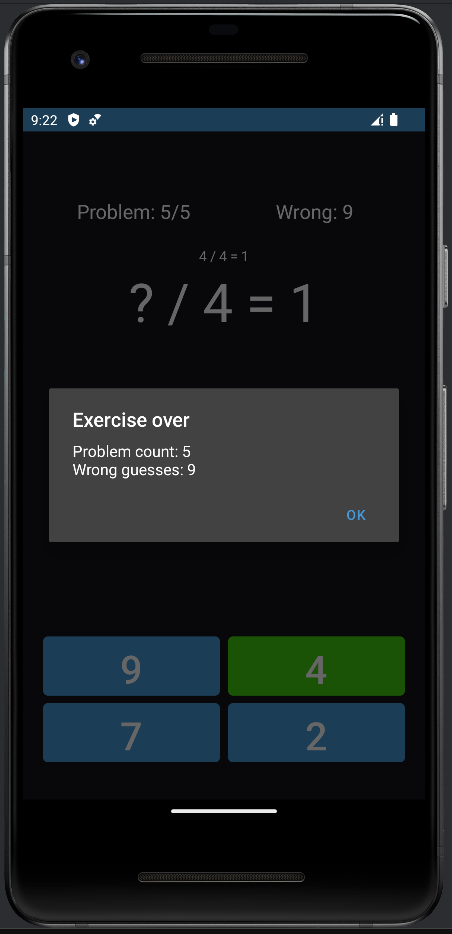
\includegraphics[height=1.7\textwidth]{img/dark_2}
			\label{fig:dark_2}
		\end{minipage}
	\end{figure}


	% ---------------------	
	% Řešené problémy
	% ---------------------	
	\chapter{Řešené problémy}
	Největší obtíž mi dělal virtuální stroj, na kterém jsem testoval aplikaci. Několikrát jsem ho musel reinstalovat a také běžel pomalu. Myslel jsem si, že to je zapříčiněno nevhodným algoritmem, ale potom když jsem spustil aplikaci na reálném zařízení, tak běžela podle představ. Při vývoji jsem proto používal hlavně svůj mobil a virtuál pouze k~testování responzivity a lokalizace rozhraní.
		
	Do nastavení jsem chtěl přidat možnost, která by uměla měnit jazyk přímo v~aplikaci. Řešení však nebylo tak přímočaré, jako u barevného schématu, protože mi nešlo určit, jaký jazyk systém preferuje. Potom jsem se dočetl, že tento přístup ani není vhodné implementovat, protože od verze Android 13 je možné zvolit lokalizaci libovolné aplikace v nastavení telefonu\footnote{\url{https://developer.android.com/guide/topics/resources/app-languages}}.

	Se samotným algoritmem, který generuje náhodné příklady, nebyly prakticky žádné problémy. Nejdéle mi trvalo sestavit finální verzi UI v editoru a ukládání/načítání parametrů \texttt{SharedPreferences}.

	% ---------------------	
	% Testování
	% ---------------------	
	\chapter{Testování}
	Aplikaci jsem testoval na virtuálních strojích Pixel 8 API 34 a Pixel 2 API 34 spolu se~svým fyzickým zařízením, které má Android 13. Zkoušel jsem očekávaný průběh cvičení, zadávání nevalidních hodnot do nastavení a jeho následné uložení a načtení. Aplikaci jsem také nainstaloval celkem na 3 telefony svých rodinných příslušníků. Ve~všech případech fungovala a vypadala podle očekávání. Její hodnocení bylo pozitivní.
	

	% ---------------------	
	% Závěr
	% ---------------------	
	\chapter{Závěr}
	Vytvořená aplikace umožňuje procvičování základních matematických operací. Jsou k~dispozici dva módy. Jeden je určený k opakovanému procvičování a druhý má podobu hry se skórem. Parametry lze měnit v nastavení a načtou se i po vypnutí aplikace. Také je možné měnit barevné schéma a případně i jazyk přes nastavení systému Android. Během testování jsem použil dva různé virtuální stroje a také několik fyzických zařízení. Aplikaci jsem vytvořit zejména pro osobní použití a jsem s ní spokojen.
	
	
	
\end{document}
